\documentclass[9pt]{beamer}

\usepackage{color, array, threeparttable}
\setbeamerfont{page number in head/foot}{size=\large}
\setbeamertemplate{footline}[frame number]
\usepackage{amsmath,amsfonts,amssymb,amsthm, gensymb}
\DeclareMathAlphabet{\mathbbold}{U}{bbold}{m}{n}    
\setbeamertemplate{footline}[frame number]
%\usepackage{beamerthemeshadow}
\usepackage[utf8]{inputenc}
\usepackage[ruled,boxed]{algorithm2e}
\makeatletter
\newcommand*{\rom}[1]{\expandafter\@slowromancap\romannumeral #1@}
\makeatother
%Information to be included in the title page:
\title{A Parallel in Time Method for Optimal Control}
\subtitle{Parareal-Based preconditioner for the BFGS algorithm}
\author{Andreas Thune}
\institute[UiO]{Faculty of Mathematics \\University of Oslo,\\Simula Research Laboratory} 

\date{Master presentation, June 2017}
\usepackage{verbatim}
\usepackage{booktabs}
\usepackage{caption,subcaption}
\usepackage{graphicx}

\usetheme{Madrid}
\usecolortheme{beaver}
%\usecolortheme{beetle}
\begin{document}
 
\frame{\titlepage}
%\tableofcontents
\begin{frame}
\frametitle{Contents}
\begin{block}{}
\centering
\alert{Goal}: Propose a parallel in time method for optimal control problems
\end{block}
\begin{itemize}
\item{Motivation:
\begin{itemize}
\item[-]{PDE constrained optimization is an important class of problems, which occur for example in: Optimal control, data assimilation and optimal design.}
\item[-]{With HPC we can improve the execution time of algorithms for optimal control.}
\item[-]{Parallelization of time-dependent PDEs often restrict parallelism to the spatial domain.}
\item[-]{Introducing parallelism in the temporal direction can increase the achievable speedup of parallel algorithms for time-dependent PDEs. }
\end{itemize}}
\item{Contents:
\begin{enumerate}[I]
%\item{The Parareal Algorithm}
\item{Optimal Control with ODE constraints}
\item{Optimization Algorithms}
\item{Presentation of our Parallel in Time Method}
\item{Experiments}
\end{enumerate}}
\end{itemize}
\end{frame}
\section{Parareal}
\begin{comment}
\begin{frame}
\frametitle{\textbf{ Part \rom{1}:}The Parareal Algorithm \rom{1}}
\begin{columns}
\column{0.48\linewidth}
\begin{itemize}
\item{The Parareal algorithm was introduced in [Lion et al.] as a way of parallelizing time-dependent PDEs in temporal direction.}
\item{The Parareal algorithm combines a coarse and a fine numerical scheme for discretization in time.}
\item{The algorithm is iterative. The fine scheme is run in parallel, while the coarse scheme is run serially.}
\end{itemize}
\column{0.48\linewidth}
\begin{figure}
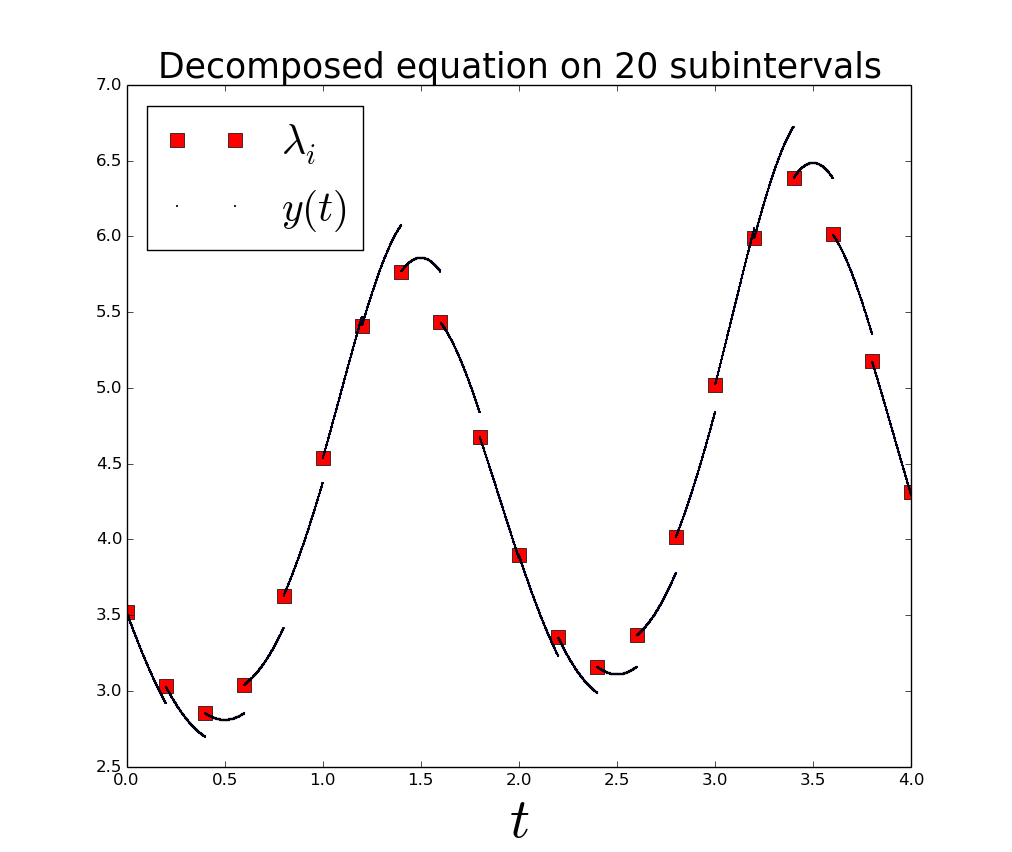
\includegraphics[scale=0.2]{parareal.png}
\caption{{\small 
The intermediate initial conditions $\{\lambda_i\}_{i=1}^{19}$ are found using a coarse solve. The fine scheme is then applied independently on each subinterval with the $\lambda_i$'s as initial conditions.
}}
\end{figure}
\end{columns}
\end{frame}
\begin{frame}
\frametitle{\textbf{ Part \rom{1}:}The Parareal Algorithm \rom{2}}
\begin{columns}
\column{0.58\linewidth}
\begin{itemize}
\item{Let $\bold{F}_{\Delta T}$ and $\bold{G}_{\Delta T}$ be the fine and coarse propagators that evolve the equation from $y(t)=\lambda$ at time $t$ to $y(t+\Delta T)$.}
\item{The predictor correction formulation of the Parareal algorithm is defined through the following iteration:
{\small \begin{align*}
\lambda_{i+1}^{k+1} &= \bold{G}_{\Delta T}(\lambda_{i}^{k+1})+\bold{F}_{\Delta T}(\lambda_{i}^{k})-\bold{G}_{\Delta T}(\lambda_{i}^{k}) \\
\lambda_0^k&=y_0,\quad \lambda_{i+1}^0 = \bold{G}_{\Delta T}(\lambda_{i}^{0})
\end{align*}}}

\end{itemize}
\column{0.38\linewidth}
\begin{figure}
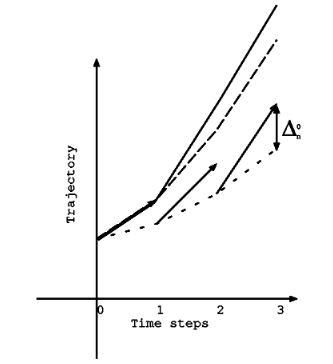
\includegraphics[scale=0.4]{parareal2.png}
\caption{Illustration of a Parareal step.}
\end{figure}
\end{columns}
\end{frame}
\end{comment}
\begin{comment}
\item{In [Maday et al] the authors show that the Parareal iteration also can be written on matrix form as:
{\small \begin{align*}
\Lambda^{k+1} = \Lambda^k -\bar M^{-1}(M\Lambda-h).
\end{align*}}
$\Lambda=\{\lambda_i\}_{i=0}^{N-1}$, $h=(y_0,0,...,0)^T$ and
\only<1>{{\small\begin{align*}
M = \left[ \begin{array}{cccc}
   \mathbbold{1} & 0 & \cdots & 0 \\  
   -\bold{F}_{\Delta T} & \mathbbold{1} & 0 & \cdots \\ 
   0 &-\bold{F}_{\Delta T} & \mathbbold{1}  & \cdots \\
   0 &\cdots &-\bold{F}_{\Delta T} & \mathbbold{1}  \\
   \end{array}  \right]\in\mathbbold{R}^{N\times N}.
\end{align*}} }
\only<2>{{\small\begin{align*}
\bar M = \left[ \begin{array}{cccc}
   \mathbbold{1} & 0 & \cdots & 0 \\  
   -\bold{G}_{\Delta T} & \mathbbold{1} & 0 & \cdots \\ 
   0 &-\bold{G}_{\Delta T} & \mathbbold{1}  & \cdots \\
   0 &\cdots &-\bold{G}_{\Delta T} & \mathbbold{1}  \\
   \end{array}  \right]\in\mathbbold{R}^{N\times N}.
\end{align*}}}}
\end{comment}
\section{Problem}
\begin{frame}
\frametitle{\textbf{ Part \rom{2}:} Optimal Control with ODE Constraints}
\begin{itemize}
\item{The focus of this thesis is ODE constrained optimization problems.}
\item{The goal of such problems is to find the state and control $(y,v)\in Y\times V$ that minimizes the objective function $J$, while simultaneously satisfying the state equation $E(y,v)=0$.}
\end{itemize}
\begin{columns}
\column{0.58\linewidth}
\begin{block}{Optimal Control Problem}
\begin{align*}
\min_{y\in Y,v\in V} &J(y(t),v), \\
\textrm{subject to} \ &E(y(t),v)=0,\quad t\in[0,T].
\end{align*}
\end{block}
\end{columns}
\end{frame}
\begin{frame}
\frametitle{\textbf{ Part \rom{2}:} The Reduced Problem}
\textbf{Reducibility}
\begin{itemize}
\item{An ODE constrained optimal control problem is called reducible if the state equation is well posed for all control variables $v\in V$.}
\item{If a problem is reducible we can define the reduced objective function $\hat{J}(v) = J(y(v),v)$.}
\item{Using $\hat J$, we can transform the optimal control problem into an unconstrained optimization problem.}
\end{itemize}
\begin{align*}
\min_{v\in V}\hat J (v)
\end{align*}
\textbf{First order optimality condition}
\begin{itemize}
\item{Since the reduced problem is unconstrained, we can use methods from unconstrained optimization to solve it. Such methods utilize the first order optimality condition $\hat J'(v)=0$, and we therefore need a way to evaluate the gradient of the reduced objective function.}
\end{itemize}
\end{frame}
\begin{frame}
\frametitle{\textbf{ Part \rom{2}:} Adjoint Approach to Gradient Evaluation}
\textbf{Deriving the gradient}
\begin{itemize}
\item<1->{If $E$ and $J$ are sufficiently smooth, and $E_y$ is continuously invertible, the gradient of the reduced objective function $\hat J'(v)$ exists.}
\item<1->{Differentiating $\hat J$ gives us: 
\begin{align*}
\hat J'(v)=D_vJ(y(v),v)=\alert<2>{y'(v)^*}J_y(y(v),v)+J_v(y(v),v)
\end{align*}}
\item<3->{\only<3-5>{Differentiating the state equation yields:} 
\only<3>{\begin{align*}
E_y(y(v),v)y'(v)+E_v(y(v),v)=0
\end{align*}}
\only<4>{\begin{align*}
y'(v)=-E_y(y(v),v)^{-1}E_v(y(v),v)
\end{align*}}
\only<5>{
\begin{align*}
y'(v)^*=-E_v(y(v),v)^*E_y(y(v),v)^{-*}
\end{align*}}
\only<6->{Define the adjoint equation:
\begin{align*}
E_y(y(v),v)^{*}p=J_y(y(v),v)
\end{align*}}}
\item<7->{Inserting the adjoint $p$ into the gradient expressions gives us:
\begin{align*}
\hat J'(v) = -E_v(y(v),v)^*p+J_v(y(v),v)
\end{align*}}
\end{itemize}
\only<8->{\textbf{Evaluating the gradient}}
\begin{itemize}
\item<8->{Evaluating $\hat J'$ for a control $v$ then comes down to the following three steps:
\begin{description}
\item[1.]{Solve the state equation $E(y,v)=0$ for $y$.}
\item[2.]{Solve the adjoint equation $E_y(y(v),v)^*p = J_y(y(v),v)$ for $p$.}
\item[3.]{Insert $y$ and $p$ into $\hat J'(v)=E_v(y(v),v)^*p +J_v(y(v),v)$.}
\end{description}}
\end{itemize}
\end{frame}
\begin{frame}
\frametitle{\textbf{ Part \rom{2}:} Example Problem}
\begin{columns}
\column{0.58\linewidth}
\begin{block}{Example Problem}
\begin{align*}
&J(y,v) = \alert<4>{\frac{1}{2}\int_0^Tv(t)^2dt} + \alert<3>{\frac{\alpha}{2}(y(T)-y^T)^2} \\
&\left\{
     \begin{array}{lr}
       	\alert<2>{y'(t)=ay(t) + \alert<4>{v(t)}}, \quad  t\in(0,T),\\
       	y(0)=y_0.
     \end{array}
   \right. 
\end{align*}
\end{block}
\begin{itemize}
\item{{\small The adjoint equation of the example problem is:}
{\small
\begin{align*}
\left\{
     \begin{array}{lr}
       	\alert<2>{p'(t)=-ap(t)}, \quad  t\in(0,T),\\
       	\alert<3>{p(T)=\alpha(y(T)-y^T)}.
     \end{array}
   \right. 
\end{align*}
}}
\item{{\small The gradient of the example objective function is:}{\small
\begin{align*}
\alert<4>{\hat{J}'(v) = v+p}
\end{align*}
}}
\item{{\small The exact solution of the example problem is:}
{\small 
\begin{align*}
v(t) = \alpha\frac{e^{aT}(y^T-e^{aT}y_0)}{1+\frac{\alpha e^{aT}}{2a}(e^{aT}-e^{-aT})}e^{-at}
\end{align*}}}
\end{itemize}
\column{0.38\linewidth}
\begin{figure}
%\centering
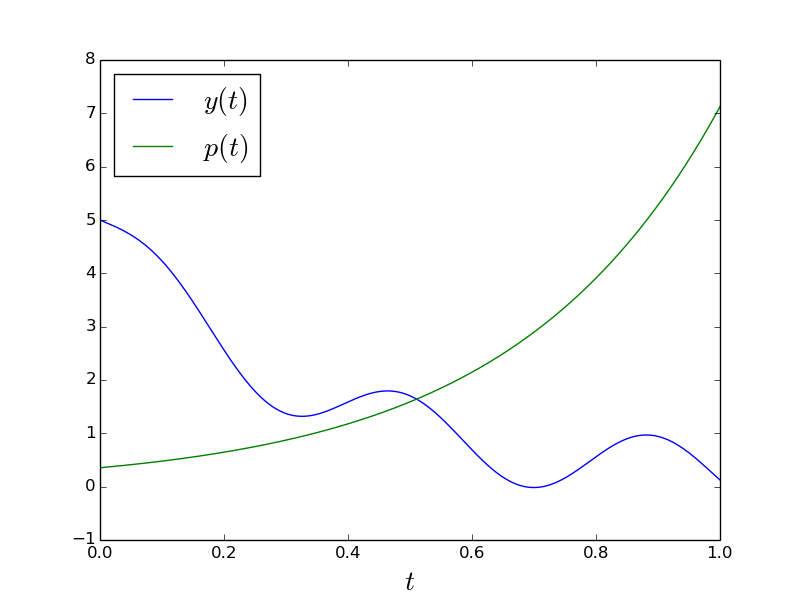
\includegraphics[scale=0.24]{ype.png}
\caption{{\tiny The state and adjoint equation of the example problem with parameters $(a,y_0,y^T,T)=(-3,5,-7,1)$, and control variable $v(t)=10\cos(5\pi t)$.}}
\end{figure}
\end{columns}
\end{frame}

\begin{frame}
\frametitle{\textbf{ Part \rom{3}:} Discretization of example problem}
\textbf{Discretizing the objective function}
%J_{\Delta t,\theta}(y,v) = \frac{\Delta t(\theta v_0^2 +(1-\theta)v_n^2)}{2}+\frac{\Delta t}{2}\sum_{i=1}^{n-1}v_n^2dt + \frac{\alpha}{2}(y_n-y^T)^2
\begin{itemize}
\item{The discrete gradient is:{\small\begin{align*}
J_{\Delta t,\theta}(y,v) = \frac{\Delta t}{2}[\theta v_0^2 +(1-\theta)v_n^2+\sum_{i=1}^{n-1}v_n^2dt] + \frac{\alpha}{2}(y_n-y^T)^2
\end{align*}
}}
\item{$\theta=0,1,\frac{1}{2}$ yields the right- and left-hand rectangle rule and the trapezoid rule.}
\end{itemize}
\textbf{Discretizing the state and adjoint equations}
\begin{itemize}
\item{We discretize the state using the $\theta$ scheme.
{\small\begin{align*}
\left\{
     \begin{array}{lr}
	\frac{y_i-y_{i-1}}{\Delta t} = \theta(ay_{i-1} +v_{i-1})+(1-\theta)(ay_i +v_i),\quad i=1,...,n\\
	y_{i=0}=y_0
	\end{array}
   \right. 
\end{align*}
}}
\item{Discrete adjoint adjoint equation:{\small\begin{align*}
\left\{
     \begin{array}{lr}
	\frac{p_i-p_{i-1}}{\Delta t} = -a(\theta p_i+(1-\theta)p_{i-1}),\quad i=0,...,n-1\\
	p_{n}=\alpha(y_n-y^T)
	\end{array}
   \right.
\end{align*}}}
\item<2>{Gradient of discrete objective function:
{\small\begin{align*}
\hat J_{\Delta t,0}'(v) = \Delta t(\mathcal{M}_{0}v+\mathcal{B} p),\quad \hat J_{\Delta t,1}'(v) = \Delta t(\mathcal{M}_{1}v+\mathcal{B}^T p)
\end{align*}}
{\small
\begin{align*}
\mathcal{M}_{\theta}=\left[ \begin{array}{cccc}
   \theta &0&  \cdots & 0 \\  
   0 & 1  & 0&\cdots \\ 
   \cdots &0 & 1 &\cdots  \\
   0 &\cdots & 0 &1-\theta \\
   \end{array}  \right],
\mathcal{B} = \left[ \begin{array}{cccc}
   0 & 0& \cdots & 0 \\  
   1 & 0 &0 & \cdots \\ 
   0 &1   & \cdots& 0 \\
   0 & 0 & 1 & 0 \\
   \end{array}  \right]\in\mathbbold{R}^{n+1\times n+1}.
\end{align*}}
}

\end{itemize}

\end{frame}

%llllllllllllllllllllllllllllllllllllllllllllllll
\section{optimization}
\begin{frame}
\frametitle{\textbf{ Part \rom{3}:} Optimization algorithms}
\begin{columns}
\column{0.58\linewidth}
\textbf{Line search methods}
\begin{itemize}
\item{Line search methods are iterative methods for solving unconstrained optimization of type:
\begin{align*}
\min_{x\in\mathbbold{R}^n}f(x).
\end{align*}}
\item{Produces iterates $\{x^k\}$, utilizing an initial guess $x^0$.}
\item{Finding $x^{k+1}$ is done using the following steps: {\small
\begin{align*}
1.\quad& \textrm{Find descent direction $p^k$.}\\
2.\quad& \textrm{Find an adequate step length $\gamma^k$.}\\
3.\quad& \textrm{Update iterate $x^{k+1} = x^k +\gamma^k p^k$.}
\end{align*}
}%
}
\item{One strategy for determining the step length $\gamma^k$ is to use the Wolfe conditions:
{\small \begin{align*}
f(x^k + \gamma_kp_k)&\leq f(x^k) + c_1\gamma_k\nabla f(x^k)\cdot p_k, \\
\nabla f(x^k + \gamma_kp_k) \cdot p_k &\geq c_2 \nabla f(x^k)\cdot p_k.
\end{align*}}}
\end{itemize}
\column{0.38\linewidth}
\begin{figure}[!h]
\centering
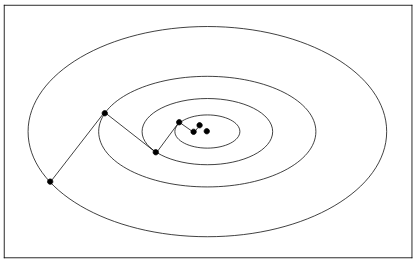
\includegraphics[scale=0.3,angle=90]{SD.png}
\caption{Illustration of the steepest descent algorithm from [Nocedal et al]. The steepest descent algorithm uses $p^k=-\nabla f(x^k)$.}
\end{figure}
\end{columns}
\end{frame}
\begin{frame}
\frametitle{\textbf{ Part \rom{3}:} Quasi Newton Methods and the BFGS Algorithm}
\textbf{Quasi-Newton methods}
\begin{itemize}
\item{Newtons method is a line search method, which uses $p^k=-\nabla^2f(x^k)^{-1}\nabla f(x^k)$.}
\item{Quasi-Newton methods use $p^k=-H^k\nabla f(x^k)$, where $H^k\approx \nabla^2f(x^k)^{-1}$.}
\end{itemize}
\begin{columns}
\column{0.58\linewidth}
\textbf{The BFGS method}
\begin{itemize}
\item{The BFGS algorithm approximates $\nabla^2f(x^k)^{-1}$ using formula:{\small
\begin{align*}
H^{k+1} &= (\mathbbold{1}-\rho_kS_k^T Y_k)H^k(\mathbbold{1} -\rho_kY_k^T S_k) + S_k^T S_k\\
S_k &= x^{k+1}-x^{k},
\quad Y_k = \nabla f(x^{k+1})-\nabla f(x^{k}),\\
\rho_k &= \frac{1}{Y_k^T S_k}\quad H^0=\mathbbold{1}.
\end{align*}
}
}
\item{If $H^k$ is symmetric positive definite so is $H^{k+1}$. }
\item{In the L-BFGS algorithm $H^{k+1}$ is calculated with a limited number of previous $H^i$'s.}
\end{itemize}
\column{0.38\linewidth}
{\small
\begin{algorithm}[H] 
\KwData{Choose an initial guess $x^0$ and a tolerance $\tau$}
\While{$||\nabla f(x^k)||\geq \tau$ }{
$x^{k+1} \leftarrow x^k - \gamma^k H^k \nabla f(x^k)$\;
Update $H^{k+1}$\;
}
\caption{The BFGS method\label{SEQ_ALG}}
\end{algorithm}
}
\end{columns}
\end{frame}
%llllllllllllllllllllllllllllllllllllllllllllllll
\section{PPC}
\begin{frame}
\frametitle{\textbf{ Part \rom{4}:} Parallelizing function and gradient evaluation}
\textbf{The Decomposed Problem}
\begin{itemize}
\item{To introduce parallelism we decompose the time domain and state equation, and define intermediate initial conditions $\Lambda=\{\lambda_i\}_{i=1}^{N-1}$.}
\item{This produces the decomposed problem.}
\end{itemize}
\begin{columns}
\column{0.48\linewidth}{\small
\begin{block}{Decomposed optimal control problem}
\begin{align*}
\min_{v,\Lambda} &\hat J(v,\Lambda), \\
\textrm{subject to} \ &y_i(T_i)=\lambda_i,i=1,...,N-1. 
\end{align*}
\end{block}}
\only<2->{\textbf{Penalized objective function}}
\begin{itemize}
\item<2->{We remove the constraints by defining the penalized objective function:{\small
\begin{align*}
\hat{J}_{\mu}(v,\Lambda) = \hat{J}(v) + \frac{\mu}{2}\sum_{i=1}^{N-1}(y_{i}(T_i)-\lambda_i)^2.
\end{align*}}}
\item<3->{The gradient of $\hat{J}_{\mu}$ is:{\small
\begin{align*}
\hat J_{\mu}'(v,\Lambda) = (v+p,\{p_{i+1}(T_i)-p_{i}(T_i)\}_{i=1}^{N-1})
\end{align*}}}
\end{itemize}
\column{0.48\linewidth}
\only<1-3>{\begin{figure}
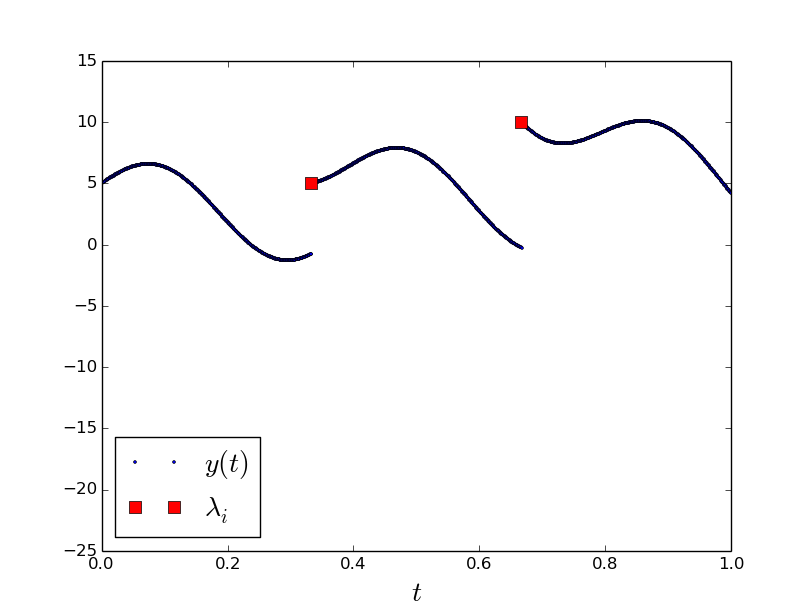
\includegraphics[trim=2cm 0 0 1.25cm,clip=true,scale=0.3]{decomp1.png}
\caption{{\tiny The decomposed state equation of the example problem with parameters $(a,y_0,y^T,T,N,\mu)=(-3,5,-7,1,3,2)$, and control variable $v(t)=50\cos(5\pi t)$ and $\Lambda=(5,10)$.}}

\end{figure}}
\only<4>{\begin{figure}
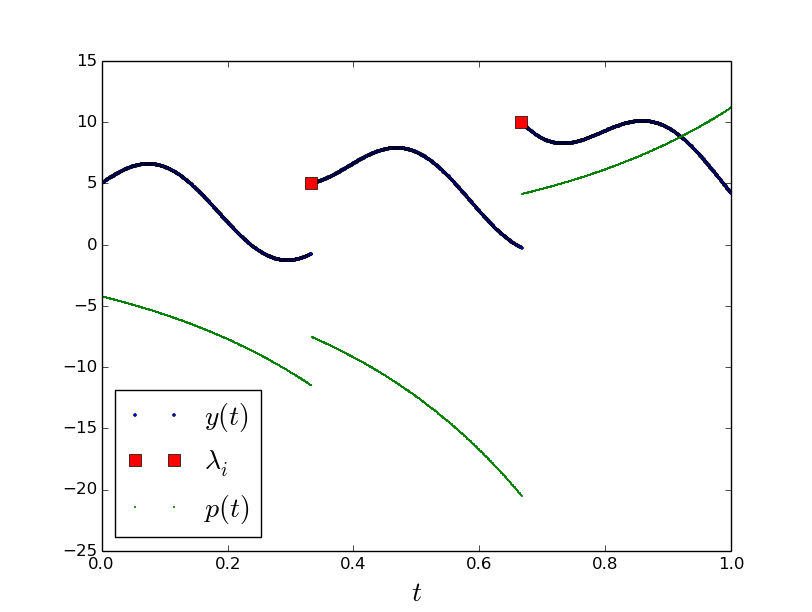
\includegraphics[trim=2cm 0 0 1.25cm,clip=true,scale=0.3]{decomp.png}
\caption{{\tiny The decomposed state and adjoint equation of the example problem with parameters $(a,y_0,y^T,T,N,\mu)=(-3,5,-7,1,3,2)$, and control variable $v(t)=50\cos(5\pi t)$ and $\Lambda=(5,10)$.}}
\end{figure}}
\end{columns}
\end{frame}
\begin{frame}
\frametitle{\textbf{ Part \rom{4}:} Parallel in Time Algorithm for Optimal Control}
\textbf{Quadratic penalty framework}
\begin{columns}
\column{0.55\linewidth}
{\tiny
\begin{algorithm}[H] 
%\TitleOfAlgo{Quadratic penalty method with preconditioned BFGS optimization}
\KwData{Choose $\mu_0,\tau_0>0$, and some initial control $(v^0,\Lambda^0$)}
\For{$k=1,2,...$}{
$(v_0^k,\Lambda_0^k) \leftarrow (v^{k-1},\Lambda^{k-1})$\;
$H^0 \leftarrow Q(\Lambda_0^{k})$\;
\While{$||\hat J'_{\mu_{k-1}}(v_j^k,\Lambda_j^k)||\geq \tau_{k-1}$ }{
\alert<2>{$\alert<6>{(v_{j+1}^k,\Lambda_{j+1}^k)} \leftarrow (v_j^k,\Lambda_j^k) - \alert<5>{\rho^j} \alert<4>{H^j} \alert<3>{\hat J'_{\mu_{k-1}}(v_j^k,\Lambda_j^k)} $}\;
Update $H^{j+1}$\;
$H^0 \leftarrow Q(\Lambda_{j+1}^k)$\;
}
$(v^{k},\Lambda^{k})\leftarrow(v_{j}^k,\Lambda_{j}^k)$\;
\eIf{STOP CRITERION on $(v^{k},\Lambda^{k})$ satisfied}{
$\bold{Stop}$ algorithm\;
}{
Choose new $\tau_k\in(0,\tau_{k-1})$ and $\mu_k\in(\mu_{k-1},\infty) $\;
}
}
\renewcommand{\thealgocf}{2}
\caption{Quadratic penalty method with BFGS optimization}
\end{algorithm}
}
\column{0.45\linewidth}
\only<2->{\textbf{BFGS step}}
\begin{itemize}
\item<2->{The optimization steps  of algorithm 3 consists of four steps:{\small
\begin{align*}
\only<3->{&1.\quad \textrm{Evaluate $J'_{\mu_{k-1}}(v_j^k,\Lambda_j^k)$.}}\\
\only<4->{&2.\quad \textrm{Apply $H^j$.}}\\
\only<5->{&3.\quad \textrm{Find step length $\rho^j$.}}\\
\only<6->{&4.\quad \textrm{Update $(v_{j+1}^k,\Lambda_{j+1}^k)$.}}
\end{align*}}}
\item<7>{Optimizing $\hat J_{\mu}$ is more difficult than optimizing $\hat J$.}
\end{itemize}
\end{columns}
\end{frame}
\begin{comment}
\begin{frame}
\frametitle{\textbf{ Part \rom{4}:} Quadratic Penalty Method \rom{1}}
\begin{itemize}
\item{Consider the constrained optimization problem:
\begin{align*}
\min_x f(x) \quad \textrm{subject to} \ c_i(x)=0 \quad i=1,...,N
\end{align*}}
\item{The quadratic penalty method is a method for solving constrained problems. The idea is to move the constraints into the functional:
\begin{align*}
f_{\mu}(x) = f(x) + \frac{\mu }{2}\sum_{i=1}^N c_i(x)^2, \quad \mu>0.
\end{align*}}
\item{The complete penalty algorithmic framework for constrained optimization is presented in algorithm 2.}
\end{itemize}
\begin{columns}
\column{0.48\linewidth}
{\tiny
\begin{algorithm}[H] 
\KwData{Choose $\mu_0,\tau_0>0$, and some initial $x^0$}
\For{$k=1,2,...$}{
Find $x^k$ s.t. $\parallel\nabla f_{\mu_{k-1}}(x^k)\parallel<\tau_{k-1}$\;
\eIf{STOP CRITERION satisfied}{
$\bold{Stop}$ algorithm\;
}{
Choose new $\tau_k\in(0,\tau_{k-1})$ and $\mu_k\in(\mu_{k-1},\infty) $\;
}
}
\caption{Penalty method\label{PEN_ALG}}
\end{algorithm}}%
\end{columns}
\end{frame}
\begin{frame}
\frametitle{\textbf{ Part \rom{4}:} Quadratic Penalty Method \rom{2}}
\begin{columns}
\column{0.48\linewidth}
\begin{itemize}
\item{The penalized objective function for the decomposed optimal control problem is {\tiny
\begin{align*}
\hat{J}_{\mu}(v,\Lambda) = \hat{J}(v) + \frac{\mu}{2}\sum_{i=1}^{N-1}(y_{i}(T_i)-\lambda_i)^2
\end{align*}}}
\item{Using the adjoint approach we can find the gradient of the penalized objective function: {\tiny
\begin{align*}
\hat J_{\mu}'(v,\Lambda) = (v+p,\{p_{i+1}(T_i)-p_{i}(T_i)\}_{i=1}^{N-1})
\end{align*}}}
\item{When we decompose the time domain and state equation, the adjoint equation is also defined independently on each subinterval.}
\end{itemize}
\column{0.48\linewidth}
\begin{figure}
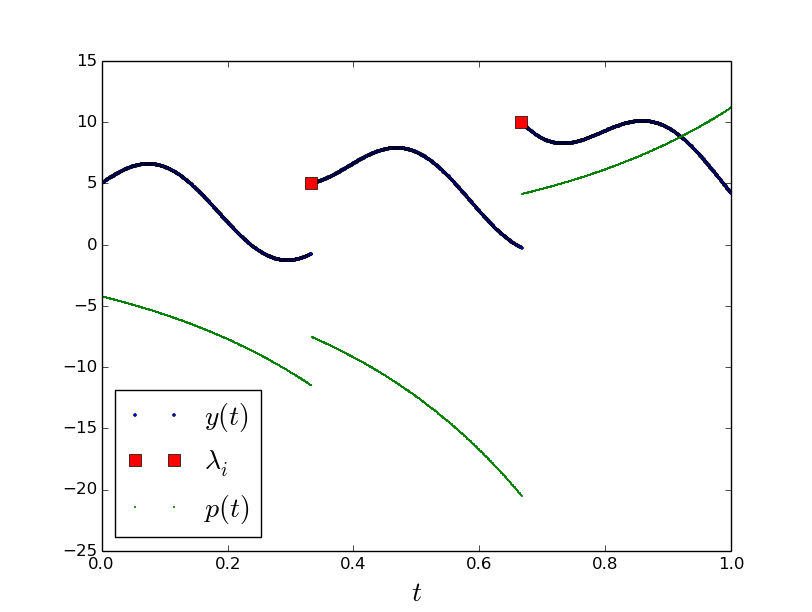
\includegraphics[scale=0.3]{decomp.png}
\caption{{\tiny The decomposed state and adjoint equation of the example problem with parameters $(a,y_0,y^T,T,N,\mu)=(-3,5,-7,1,3,2)$, and control variable $v(t)=50\cos(5\pi t)$ and $\Lambda=(5,10)$.}}
\end{figure}
\end{columns}
\end{frame}
\end{comment}
\begin{frame}
\frametitle{\textbf{ Part \rom{4}:} Parareal-Based Preconditioner}
\textbf{Preconditioning the BFGS method}
\begin{itemize}
\item{We want to use the preconditioner proposed in [Maday et al] in the BFGS method. We do this by setting $H_0=Q$, where $Q$ is: {\small
\begin{align*}
Q = \left[ \begin{array}{cc}
	\mathbbold{1} & 0 \\
	0 & Q_{\Lambda} \\
	\end{array} \right]\in \mathbb{R}^{n_v+N-1\times n_v+N-1},\quad Q_{\Lambda}\in\mathbb{R}^{N-1\times N-1}
\end{align*}}}
\item<1->{We want $Q$ to have the following properties:\begin{itemize}
\item<1->[1.]{$Q$ should approximate the Hessian of $\hat J_{\mu}$.}
\item<1->[2.]{$Q$ must be symmetric positive definite.}
\item<1->[3.]{Applying $Q$ should be a cheap operation.}
\end{itemize}
}
\end{itemize}
\textbf{The virtual problem}
\begin{itemize}
\item{We derive and motivate $Q_{\Lambda}$ by considering the virtual problem.}
\end{itemize}
\begin{columns}
\column{0.58\linewidth}
\begin{block}{Virtual problem}
{\small\begin{align*}
\min_{y,\Lambda}&\bold J(y,\Lambda)\quad \textrm{Seubject to:}\ E(y,\Lambda)=0 \\
&\bold J(y,\Lambda)=\frac{1}{2}\sum_{i=1}^{N-1}(y_i(T_i)-\lambda_i)^2
\end{align*}}
\end{block}
\end{columns}
\end{frame}
\begin{frame}
\frametitle{\textbf{ Part \rom{4}:} Virtual Problem \rom{1}}
\textbf{Fine and coarse propagators}
\begin{itemize}
\item{Define $\bold{F}_{\Delta T}$ and $\bold{G}_{\Delta T}$ to be operators that evolve the state equation from $\lambda_i$ at time $T_{i}$ to $y_i(T_{i}+\Delta T)$ using a fine or a coarse numerical scheme. }
\end{itemize}
\textbf{Least squares formulation}
\begin{itemize}
\item{We can write the reduced virtual objective function as a least squares function:
{\small
\begin{align*}
\bold{ \hat J}(\Lambda) = \frac{1}{2} x(\Lambda)^Tx(\Lambda),\quad
x(\Lambda)=\left( \begin{array}{c}  
   \lambda_1 - \bold F_{\Delta T}(y_0) \\ 
   \lambda_2 - \bold F_{\Delta T}(\lambda_1) \\
   \cdots  \\
   \lambda_{N-1} -\bold F_{\Delta T}(\lambda_{N-1}) \\
   \end{array}  \right).
\end{align*}}}
\item{The gradient of the virtual objective function is:
{\small
\begin{align*}
\nabla \bold{\hat J}(\Lambda)= \nabla x(\Lambda)^T x(\Lambda) = M(\Lambda)^Tx(\Lambda),
\end{align*}}
where 
{\small
\begin{align*}
M(\Lambda)= \left[ \begin{array}{cccc}
   1 & 0 & \cdots & 0 \\  
   -\bold{F}_{\Delta T}'(\lambda_{1}) & 1 & 0 & \cdots \\ 
   0 &-\bold{F}_{\Delta T}'(\lambda_{2}) & 1  & \cdots \\
   0 &\cdots &-\bold{F}_{\Delta T}'(\lambda_{N-1}) & 1  \\
   \end{array}  \right]\in\mathbbold{R}^{N-1\times N-1}
\end{align*}}}
\end{itemize}
\end{frame}
\begin{frame}
\frametitle{\textbf{ Part \rom{4}:} Virtual Problem \rom{2}}
\textbf{Virtual Hessian}
\begin{itemize}
\item{When the state equation is linear the Hessian of the virtual objective function is:
{\small 
\begin{align*}
\nabla^2 \bold{\hat J}(\Lambda)&= \nabla x(\Lambda)^T \nabla x(\Lambda) + \nabla^2 x(\Lambda)^Tx(\Lambda) \\
&= M(\Lambda)^TM(\Lambda).
\end{align*}}}
\item<2->{$M(\Lambda)^TM(\Lambda)$ is a symmetric positive definite matrix.}
\end{itemize}
\only<3->{\textbf{Approximating the virtual Hessian}}
\begin{itemize}
\item<3->{We base the preconditioner $Q_{\Lambda}$ on an approximation of the inverse of {$M(\Lambda)^TM(\Lambda)$}. We approximate $M(\Lambda)$ using the coarse propagator:
\begin{align*}
\bar M(\Lambda)= \left[ \begin{array}{cccc}
   1 & 0 & \cdots & 0 \\  
   -\bold{G}_{\Delta T}'(\lambda_{1}) & 1 & 0 & \cdots \\ 
   0 &-\bold{G}_{\Delta T}'(\lambda_{2}) & 1  & \cdots \\
   0 &\cdots &-\bold{G}_{\Delta T}'(\lambda_{N-1}) & 1  \\
   \end{array}  \right]\in\mathbbold{R}^{N-1\times N-1}
\end{align*}}
\item<4->{$Q_{\Lambda}=\bar{M}^{-1}(\Lambda)\bar{M}^{-T}(\Lambda)$ will be used as a preconditioner for the BFGS method.}
\end{itemize}
\end{frame}
\begin{comment}
\only<1>{{\small
\begin{align*}
\nabla^2 \bold{\hat J}(\Lambda)&= \nabla x(\Lambda)^T \nabla x(\Lambda) + \nabla^2 x(\Lambda)^Tx(\Lambda) = M(\Lambda)^TM(\Lambda) + D(\Lambda) \\
&= M(\Lambda)^TM(\Lambda) + \left[ \begin{array}{cccc}
   D_1 & 0 & \cdots & 0 \\  
   0 & D_2 & 0 & \cdots \\ 
   0 &0 & D_{N-2}  & \cdots \\
   0 &0 & 0  &0\\
   \end{array}  \right],D_i=-\bold{F}_{\Delta T}''(\lambda_i)(\lambda_{i+1}-\bold F_{\Delta T}(\lambda_i)).
\end{align*}}}
\begin{frame}
\frametitle{\textbf{ Part \rom{4}:} Applying $\bar M(\Lambda)^{-1}\bar M(\Lambda)^{-T}$}
\begin{itemize}
\item{Let $N=3$, $x,y\in \mathbbold{R}^3$ and let $\bar M(\Lambda)\in \mathbbold{R}^{3\times 3}$.
\only<1>{\begin{align*}
 \left[ \begin{array}{ccc}
   1 & 0 &  0 \\  
   -\bold{G}_{\Delta T}'(\lambda_{1}) & 1 & 0  \\ 
   0 &-\bold{G}_{\Delta T}'(\lambda_{2}) & 1   \\
   \end{array}  \right] 
   \left(\begin{array}{c} 
   x_1 \\
   x_2 \\
   x_3\\ 
\end{array}    \right) =
\left(\begin{array}{c} 
   y_1 \\
   y_2 \\
   y_3\\
\end{array}    \right)
\end{align*}}
\only<2>{\begin{align*}
\left(\begin{array}{c} 
   x_1 \\
   x_2 -\bold{G}_{\Delta T}'(\lambda_1)x_1\\
   x_3-\bold{G}_{\Delta T}'(\lambda_2)x_2\\ 
\end{array}    \right) =
\left(\begin{array}{c} 
   y_1 \\
   y_2 \\
   y_3\\
   \end{array}    \right)
\end{align*}}
\only<3>{\begin{align*}
\left(\begin{array}{c} 
   x_1 \\
   x_2 \\
   x_3\\ 
\end{array}    \right) =
\left(\begin{array}{c} 
   y_1 \\
   y_2 +\bold{G}_{\Delta T}'(\lambda_1)x_1\\
   y_3+\bold{G}_{\Delta T}'(\lambda_2)x_2\\
   \end{array}    \right)
\end{align*}}
\only<4->{\begin{align*}
\left(\begin{array}{c} 
   x_1 \\
   x_2 \\
   x_3\\ 
\end{array}    \right) =
\left(\begin{array}{c} 
   y_1 \\
   y_2 +\bold{G}_{\Delta T}'(\lambda_1)y_1\\
   y_3+\bold{G}_{\Delta T}'(\lambda_2)( y_2 +\bold{G}_{\Delta T}'(\lambda_1)y_1)\\
   \end{array}    \right) = \bar M(\Lambda)^{-1}\left(\begin{array}{c} 
   y_1 \\
   y_2 \\
   y_3\\
   \end{array}    \right)
\end{align*}}}
\item<4->{Applying $\bar M(\Lambda)^{-1}$ to a vector is the same as applying the linearised forward model.}
\item<5->{If $\bold{G}_{\Delta T}$ is a cheap evaluating $\bar M(\Lambda)^{-1}y$ requires $\mathcal{O}(N-1)$ operations.}
\end{itemize}
\end{frame}
\end{comment}
\begin{comment}
\begin{frame}
\frametitle{\textbf{ Part \rom{4}:} Properties of $\bar M(\Lambda)^T\bar M(\Lambda)$}
\begin{columns}
\column{0.48\linewidth}
\begin{itemize}
\item{The inverse of $\bar M(\Lambda)$ is a linearised forward solve, while the inverse of $\bar M^T(\Lambda)$ is a linearised backwards solve.}
\item{For $N=2$ decompositions of the time domain $Q=\mathbbold{1}$.}
\item{Applying $Q$ is an $\mathcal{O}(N)$ operation.}
\end{itemize}
\column{0.58\linewidth}
\centering
\begin{figure}[!h]
\centering
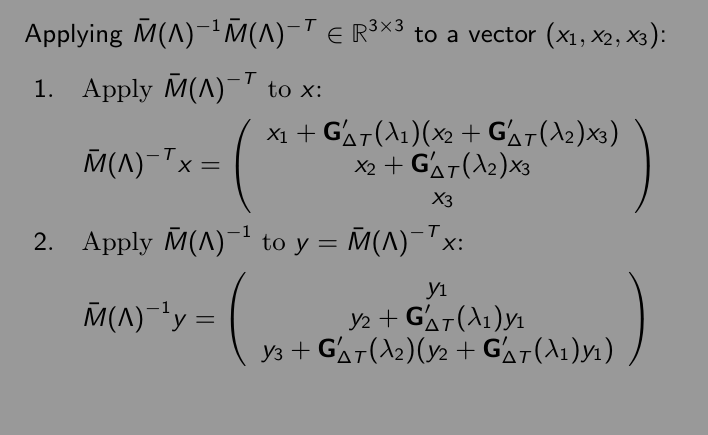
\includegraphics[scale=0.24]{apply.png}
\end{figure}
\end{columns}
\end{frame}
\end{comment}
\begin{comment}
{\tiny
Applying $\bar M(\Lambda)^{-1}\bar M(\Lambda)^{-T}\in \mathbbold{R}^{3\times 3}$ to a vector $(x_1,x_2,x_3)$:
\begin{align*}
1.\quad &\textrm{Apply $\bar M(\Lambda)^{-T}$ to $x$:} \\
&\bar M(\Lambda)^{-T}x= \left(\begin{array}{c}
x_1 + \bold G_{\Delta T}'(\lambda_1)(x_2 + \bold G_{\Delta T}'(\lambda_2)x_3)\\
x_2 + \bold G_{\Delta T}'(\lambda_2)x_3 \\
x_3 \\
\end{array}
\right) 
\\
2.\quad &\textrm{Apply $\bar M(\Lambda)^{-1}$ to $y=\bar M(\Lambda)^{-T}x$:} \\
&\bar M(\Lambda)^{-1}y = \left(\begin{array}{c}
y_1 \\
y_2 + \bold G_{\Delta T}'(\lambda_1)y_1 \\
y_3 + \bold G_{\Delta T}'(\lambda_2)(y_2 + \bold G_{\Delta T}'(\lambda_1)y_1)\\
\end{array}
\right)
\end{align*}}
\end{comment}
\begin{comment}
\begin{frame}
\centering
Applying $\bar M(\Lambda)^{-1}\bar M(\Lambda)^{-T}\in \mathbbold{R}^{3\times 3}$ to a vector $(x_1,x_2,x_3)$:
\begin{align*}
1.\quad &\textrm{Apply $\bar M(\Lambda)^{-T}$ to $x$:} \\
&\bar M(\Lambda)^{-T}x= \left(\begin{array}{c}
x_1 + \bold G_{\Delta T}'(\lambda_1)(x_2 + \bold G_{\Delta T}'(\lambda_2)x_3)\\
x_2 + \bold G_{\Delta T}'(\lambda_2)x_3 \\
x_3 \\
\end{array}
\right) 
\\
2.\quad &\textrm{Apply $\bar M(\Lambda)^{-1}$ to $y=\bar M(\Lambda)^{-T}x$:} \\
&\bar M(\Lambda)^{-1}y = \left(\begin{array}{c}
y_1 \\
y_2 + \bold G_{\Delta T}'(\lambda_1)y_1 \\
y_3 + \bold G_{\Delta T}'(\lambda_2)(y_2 + \bold G_{\Delta T}'(\lambda_1)y_1)\\
\end{array}
\right)
\end{align*}
\end{frame}
\end{comment}

\begin{frame}
\frametitle{\textbf{ Part \rom{5}:} Verification \rom{1}}
\begin{columns}
\column{0.58\linewidth}
\begin{block}{Test Problem \rom{1}}
We verify parts of our algorithm using the below defined problem with $T=1$
{\small\begin{align*}
&J(y,v) = \frac{1}{2}\int_0^{T}v(t)^2dt + \frac{1}{2}(y(T)-11.5)^2, \\
&\left\{
     \begin{array}{lr}
       	y'(t)=-3.9y(t) + v(t) \quad t\in(0,T)\\
       	y(0)=3.2
     \end{array}
   \right. 
\end{align*}}
\end{block}
\end{columns}
\begin{itemize}
\item{Verify the discrete gradients using the Taylor test.}
\item{Verify the convergence of the serial solver.}
\item{Verify the performance of the parallel objective function and gradient evaluations.}
\item{Verify the consistency of our parallel algorithm.}
\end{itemize}
\end{frame}
\begin{frame}
\frametitle{\textbf{ Part \rom{5}:} Verification \rom{2}}
\begin{columns}
\column{0.48\linewidth}
\textbf{Verifying the discrete gradients}
\begin{block}{Taylor Test}
{\small If $\hat J$ is the gradient of $J$ the following holds:}
{\small
\begin{align*}
D(\epsilon)&=|\hat J(v+\epsilon w)-\hat J(v)-\epsilon\hat J'(v)\cdot w| \\&= \mathcal{O}(\epsilon^2)
\end{align*}}
\end{block}
\begin{itemize}
\item{\small{The discrete gradient of both the penalized and unpenalized objective function is verified using the Taylor test.}}
\item{\small{We use the Crank-Nicolson scheme and the trapezoid rule with $\Delta t=0.01$.}}
\end{itemize}
\column{0.38\linewidth}
{\small
\begin{table}[h]
\centering
\caption{Taylor test applied to the discrete objective function $\hat J_{\Delta t}$.}\label{Taylor_tab1}
\begin{tabular}{lrl}
\toprule
{} $\epsilon$&   $D(\epsilon)$ &    rate \\
\midrule
1e+00 &       5.24e+03 &      -- \\
1e-01 &       5.24e+01 &      -2 \\
1e-02 &       5.24e-01 &       -2 \\
1e-05 &        5.24e-07 &      -2 \\
\bottomrule
\end{tabular}
\end{table}
}
{\small
\begin{table}[!h]
\centering
\caption{Taylor test applied to the discrete penalized objective function $\hat J_{\Delta t,\mu}$.}
\label{Taylor_tab2}
\centering
\begin{tabular}{lrl}
\toprule
{}$\epsilon$&   $D_2$ &    rate  \\
\midrule
1e+00 &         1.07e+04 &      -- \\
1e-01 &         1.07e+02 &      -2 \\
1e-03 &          1.07e-02 &      -2 \\
1e-06 &          1.07e-08 &      -2 \\
\bottomrule
\end{tabular}
\end{table}}
\end{columns}
\end{frame}
\begin{frame}
\frametitle{\textbf{ Part \rom{5}:} Verification \rom{3}}
%\hline
\begin{columns}
\column{0.48\linewidth}
\textbf{Convergence of serial algorithm}
\begin{itemize}
{\small
\item{We investigate whether the numerical solution of the serial algorithm converge to exact solution when we decrease $\Delta t$.}
}
\end{itemize}
\column{0.48\linewidth}
{\tiny
\begin{table}[!h]
\caption{{\tiny Results of serial algorithm with an implicit Euler discretization.}} \label{IE_convergence}
\centering
\begin{tabular}{lrrll}
\toprule
{} $\Delta t$&    $\frac{||v_e-v||_{\infty}}{||v||_{\infty}}$ &  $\frac{\hat J(v_e)-\hat J(v)}{\hat J(v_e)}$ & $v$ rate & $\hat J$  rate \\
\midrule
0.02000 &  0.2126 &  1.70e-02 &        -- &       -- \\
0.01000 &  0.1360 &  4.50e-03 & -0.64 & -1.92 \\
0.00100 &  0.0174 &  4.70e-05 & -0.89 & -1.98 \\
0.00010 &  0.0018 &  4.72e-07 &   -0.99 & -1.99 \\
0.00001 &  0.0002 &  4.72e-09 &  -1.00 & -1.99 \\
\bottomrule
\end{tabular}
\end{table}}
\end{columns}
\textbf{Performance of parallel function and gradient evaluation}
\begin{itemize}
{\small
\item{Our parallel algorithm can only produce a speedup if evaluating $\hat J_{\mu}(v,\Lambda)$ and $\hat J_{\mu}'(v,\Lambda)$ runs faster than evaluating $\hat J(v)$ and $\hat J '(v)$.}
\item{We investigate this evaluating the different functions and gradients in context of the test problem with $\Delta t= 10^{-7}$ and an implicit Euler discretization. }}
\end{itemize}
{\tiny
\begin{table}[!h]
\centering
\begin{tabular}{lrrrr}
\toprule
{}$N$ &  functional time (s) &  gradient time (s) &  functional speedup &  gradient speedup \\
\midrule
1 &           8.350 &         14.930 &            1.000 &          1.000 \\
3 &           2.932 &          5.033 &            2.847 &          2.966 \\
5 &           1.796 &          3.089 &            4.647 &          4.833 \\
\bottomrule
\end{tabular}
\end{table}}
\end{frame}
%llllllllllllllllllllllllllllllllllllllllllllllllll
\section{consistency}
\begin{frame}
\frametitle{\textbf{ Part \rom{5}:} Consistency}
\begin{columns}
\column{0.48\linewidth}
\textbf{Test description}
\begin{itemize}
\item{We solve the test problem with $N=2$, $\Delta t=10^{-2}$ and a Crank-Nicolson discretization.}
\item{We compare the result of the serial an parallel algorithm. }
\end{itemize}
\textbf{Theoretical background}
\begin{itemize}
\item{Results must be viewed in context of the theory of the penalty framework.}
\end{itemize}
\begin{block}{Theorem 1}
If $(v^k,\Lambda^k)$ is the exact global minimizer of $\hat J_{\mu_{k}}$ $\forall$ $k$, the iterates of the penalty method will converge to the minimizer of $\hat J$.
\end{block}
\only<2>{\begin{block}{Theorem 2}
The iterates of the penalty framework will at least converge to a feasible point.
\end{block}}
\column{0.48\linewidth}
\begin{figure}[!h]
\centering
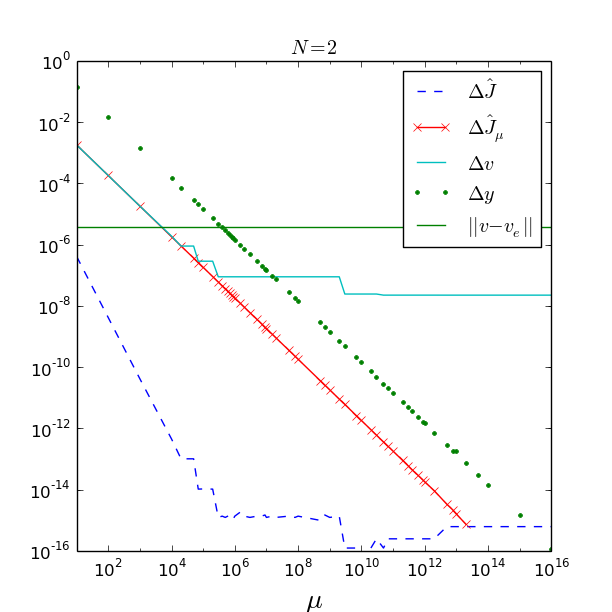
\includegraphics[scale=0.35]{con2.png}
\caption{{\tiny Results of consistency test. $\Delta \hat J=|\hat J(v_p)-\hat J(v_s)|$, $\Delta v = ||v_p-v_s||$ and $\Delta y=\max\{y_i(T_i)-y_{i+1}(T_i)\}$. }}
\end{figure}
\end{columns}
\end{frame}
%llllllllllllllllllllllllllllllllllllllllllllllllll
\section{Experiments}
\begin{frame}
\frametitle{\textbf{ Part \rom{5}:} Experimental Setup}
\begin{columns}
\column{0.58\linewidth}
\begin{block}{Test Problem \rom{2}}
We investigate our algorithm using the below defined problem with $T=100$
{\small\begin{align*}
&J(y,v) = \frac{1}{2}\int_0^{T}v(t)^2dt + \frac{1}{2}(y(T)-11.5)^2, \\
&\left\{
     \begin{array}{lr}
       	y'(t)=-0.097y(t) + v(t) \quad t\in(0,T)\\
       	y(0)=3.2
     \end{array}
   \right. 
\end{align*}}
\end{block}
\begin{itemize}
\item<1->{Define $L_S$ and $L_{p_N}$ as total number of function and gradient evaluations for the serial and parallel algorithms.}
\item<1->{Ideal speedup $\hat{S}=\frac{N L_S}{L_{p_N}}$.}
\item<1->{We investigate the performance of our algorithm when for different values of $\mu$, $N$ and $n$.}
\end{itemize}
\column{0.38\linewidth}
\begin{figure}
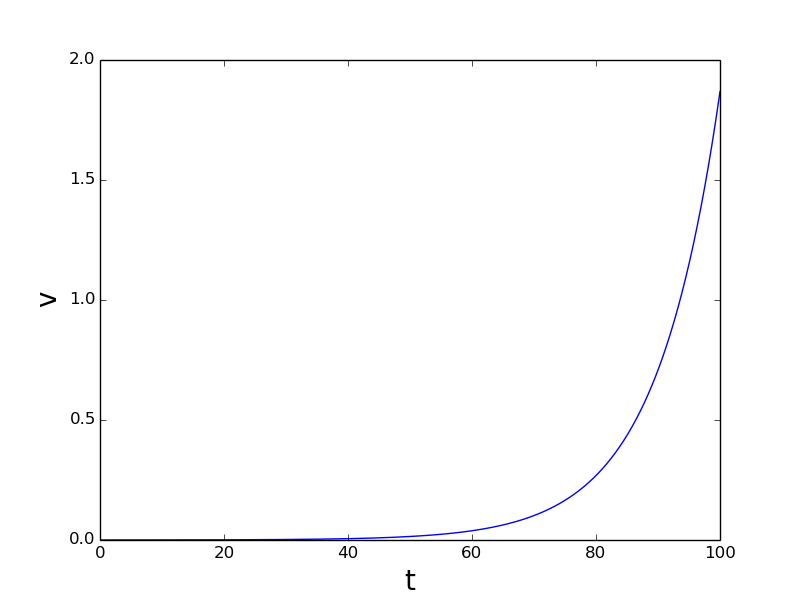
\includegraphics[scale=0.25]{exact.png}
\caption{The exact solution of the test problem.}
\end{figure}
\end{columns}
\end{frame}
\begin{comment}
\begin{frame}
\frametitle{\textbf{ Part \rom{5}:} Performance for Increasing $N$}
\begin{itemize}
\item{Test example problem for fixed problem size $n=10^5$ and penalty parameter $\mu=10^4$ for increasing number of decompositions of the time domain $N$, and an implicit Euler discretiztion of the equations.}
\item{We compare the preconditioned and unpreconditioned solver, using number of function and gradient evaluations ($L_{p_N}$), control variable error ($||v_e-v||$) and ideal speedup ($\hat{S}$).}
\end{itemize}
{\small\begin{table}[h]
\centering
\begin{tabular}{lrrllrr}
\toprule
{}$N$ &  pc $L_{p_N}$ &  non-pc $L_{p_N}$ &       $||v_e-v_{pc}||$ &  $||v_e-v||$  &  pc $\hat{S}$ &  non-pc $\hat{S}$ \\
\midrule
1   &     13 &      13 &  0.000040 &    0.000040 &    1.00 &        1.00 \\
8   &     53 &      53 &  0.000483 &    0.001725 &    1.96 &        1.96 \\
16  &    109 &     175 &  0.001612 &    0.004105 &    1.90 &        1.18 \\
32  &     97 &     361 &  0.001267 &    0.008545 &    4.28 &        1.15 \\
64  &     43 &     469 &  0.001621 &    0.017026 &   19.34 &        1.77 \\
\bottomrule
\end{tabular}
\end{table}}
\end{frame}
\end{comment}
\begin{frame}
\frametitle{\textbf{ Part \rom{5}:} Performance for Increasing $\mu$}
\textbf{Experimental parameters}
\begin{itemize}
\item{$N=16$, $n=10^3$ and Crank-Nicolson discretization.}
\item{Solve test problem with preconditioned and unpreconditioned parallel algorithm for increasing $\mu$.}
%\item{We now test the algorithm on the example problem for a fixed number of decompositions $N=16$ and number of time-steps $n=10^3$, while the penalty parameter $\mu$ is increased. This time the Crank-Nicolson scheme was used to discretize the equations.}
\end{itemize}
\textbf{Results:}
{\small\begin{table}
\centering
\begin{tabular}{lrrrrrr}
\toprule
{} $\mu$&    pc $L_{p_{16}}$ & non-pc $L_{p_{16}}$  &  pc $\hat S$ & non-pc $\hat S$ &  $||v_e-v_{pc}||$ &      $||v_e-v||$\\
\midrule
1e+2   &   \alert<2>{99} &  \alert<2>{357} &  \alert<4>{3.71} &  1.03 &  \alert<3>{6.5e-4} &   \alert<3>{6.5e-4}\\
1e+3  &  \alert<2>{153} &  \alert<2>{885} &  \alert<4>{2.40} &  0.41 &  \alert<3>{3.1e-5} &  \alert<3>{1.1e-4} \\
1e+5 &  \alert<2>{155} &  \alert<2>{379} &  \alert<4>{2.37} &  0.97 &  \alert<3>{3.9e-5} &  \alert<3>{9.2e-5} \\
\alert<5>{1e+08} &  \alert<2,5>{410} &  \alert<2,5>{3007} &  \alert<5>{0.89} &  0.12 &  \alert<3>{3.9e-5} &  \alert<3>{4.3-2} \\
\bottomrule
\end{tabular}
\end{table}}
\begin{columns}
\column{0.49\linewidth}
\only<6->{\textbf{Improved results}}
\begin{itemize}
\item<6->{We can improve the results by doing two penalty iterations.}
\end{itemize}
\column{0.49\linewidth}
\onslide<6->{{\small\begin{table}[h!]
\begin{tabular}{lrrr}
\toprule
{} $\mu$ & $L_{p_{16}}$ & $\hat S$ & $||v_e-v_{pc}||$ \\
\midrule
1e+5 &155 &2.37 &3.85e-5\\
1e+8 &25 &14.72 &3.87e-5\\
\midrule
Overall result &180 &2.04 &3.87e-5\\
\bottomrule
\end{tabular}
\end{table}}}
\end{columns}
\end{frame}
\begin{frame}
\frametitle{\textbf{ Part \rom{5}:} Results for Unsimulated Parallelism \rom{1}}
\textbf{Experimental setup}
\begin{itemize}
\item{We tested our algorithm on the Abel computer cluster.}
\item{We ran the test problem for $n=6\cdot 10^5,12\cdot 10^5,24\cdot 10^5$, and for $N$ between $2$ and $120$.}
\end{itemize}
\textbf{Results:}
\begin{columns}
\column{0.45\linewidth}
\only<1>{\begin{figure}[!h]

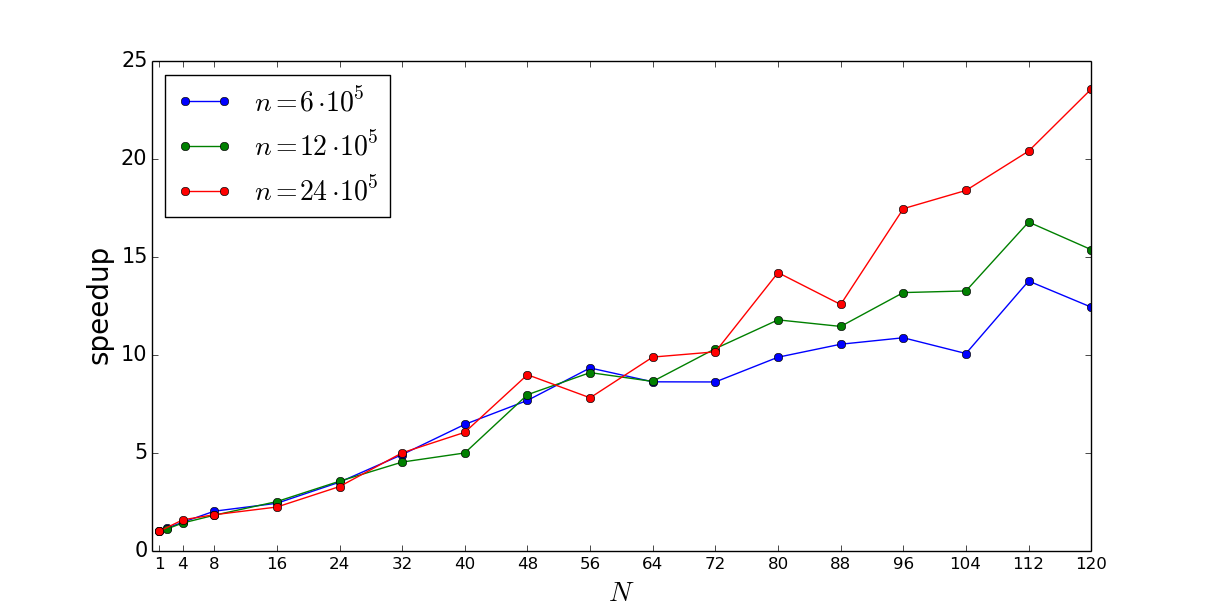
\includegraphics[trim=2cm 0 0 3.25cm,scale=0.21]{res1.png}
\end{figure}}
\only<2>{\begin{figure}[!h]

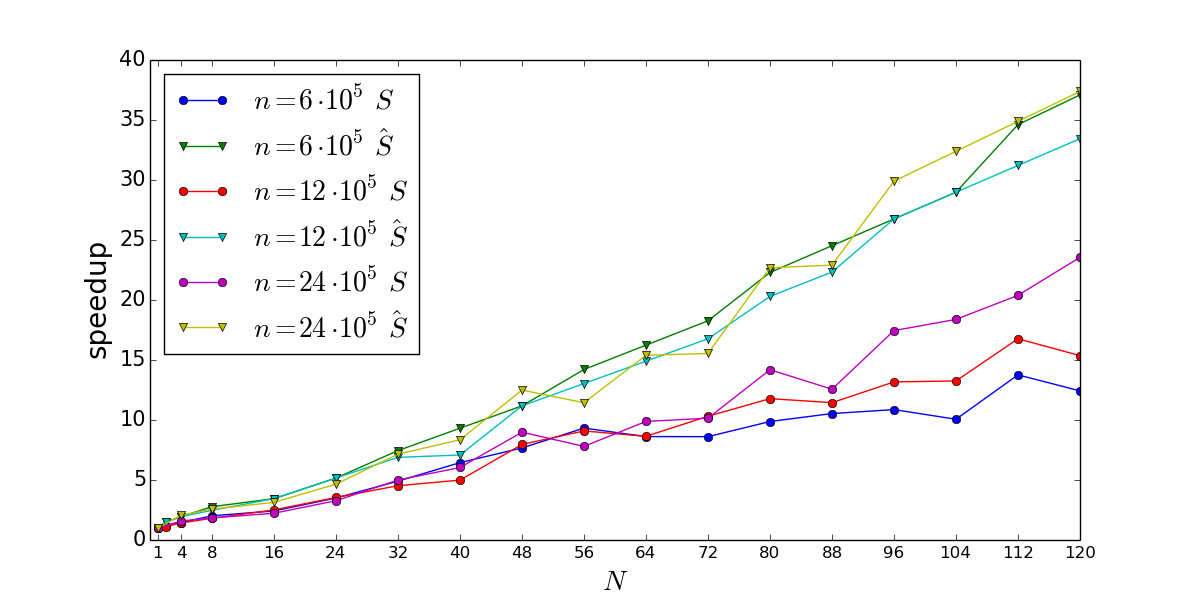
\includegraphics[trim=2cm 0 0 3.25cm,scale=0.21]{SS.png}
\end{figure}}
\column{0.45\linewidth}
\only<1>{
\begin{figure}
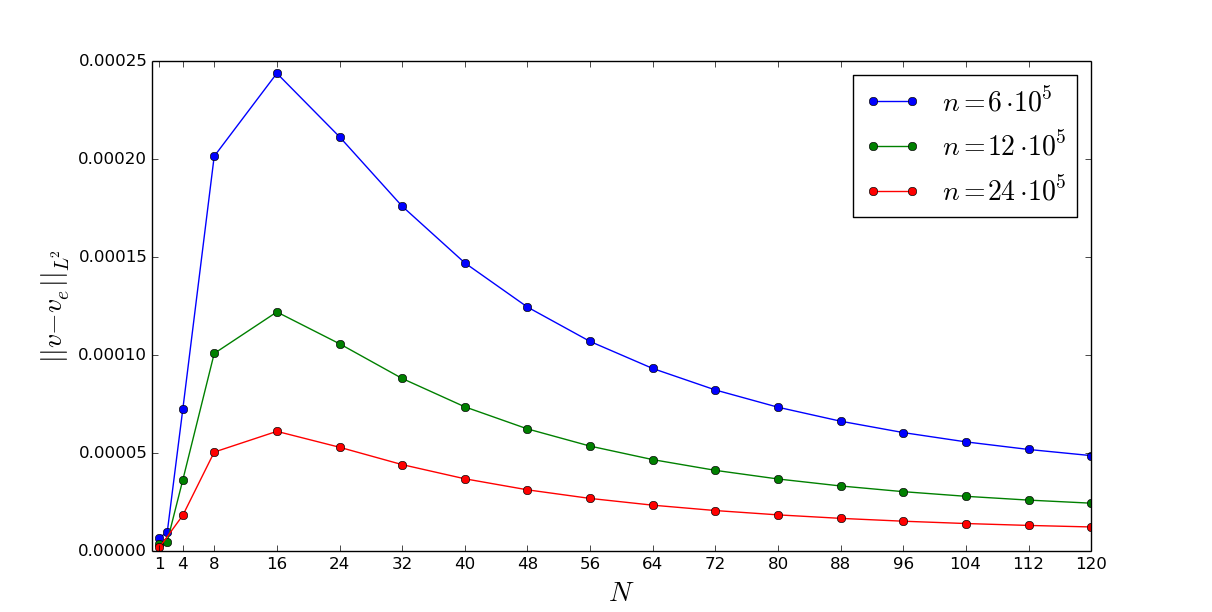
\includegraphics[trim=2cm 0 0 3.25cm,scale=0.21]{res2.png}

%\caption{Measured speedup, efficiency, error and $L_{p_N}$ for the three problem sizes. }
\end{figure}}
\only<2>{
\begin{figure}
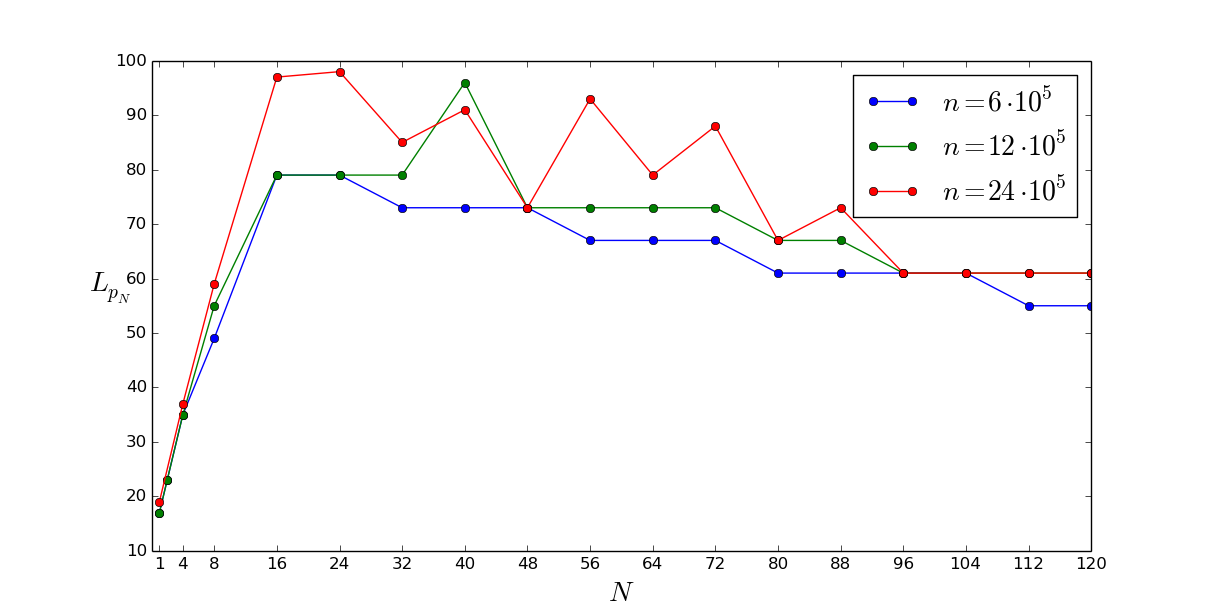
\includegraphics[trim=2cm 0 0 3.25cm,scale=0.21]{res3.png}

%\caption{Measured speedup, efficiency, error and $L_{p_N}$ for the three problem sizes. }
\end{figure}}
\end{columns}
\end{frame}
\begin{comment}
\begin{frame}
\frametitle{\textbf{ Part \rom{5}:} Results for Unsimulated Parallelism \rom{2}}
\begin{columns}
\column{0.48\linewidth}
\begin{itemize}
\item{When we compare the ideal speedup $\hat S$ with actual achieved speedup $S$ we observe that the actual speedup is lower than the ideal speedup. We also notice that disparity between $S$ and $\hat S$ grows as $N$ becomes larger.}
\item{The reason for the difference between $S$ and $\hat S$ is parallel overhead.}
\end{itemize}
\column{0.48\linewidth}
\begin{figure}
\centering
\begin{subfigure}{1\linewidth}
\centering
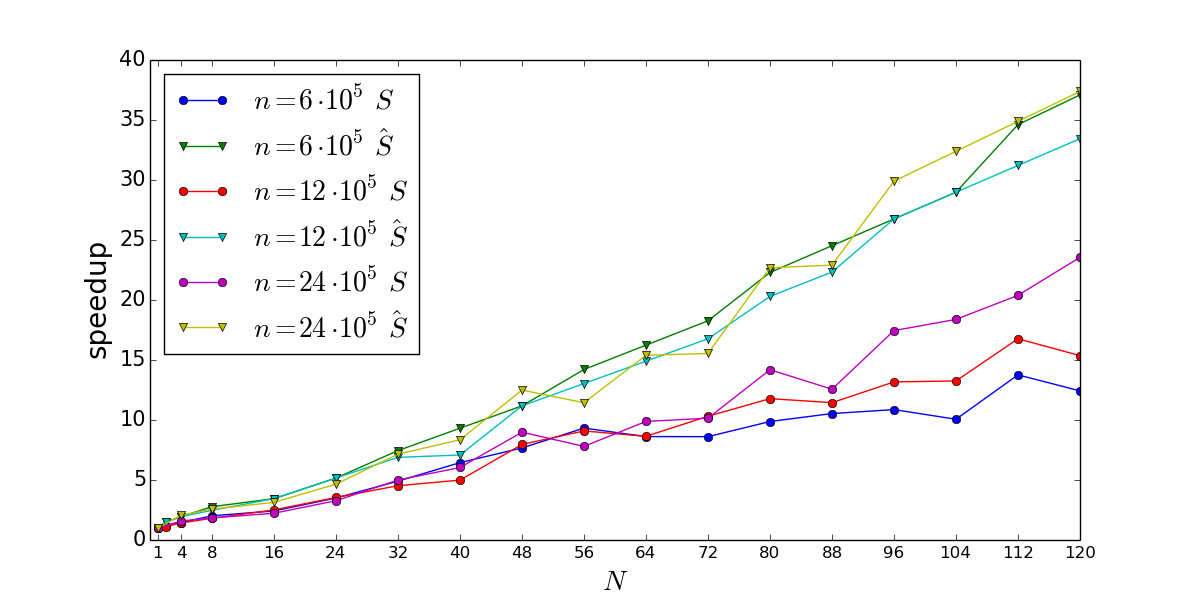
\includegraphics[scale=0.2]{SS.png}
\end{subfigure}
\\
\begin{subfigure}{1\linewidth}
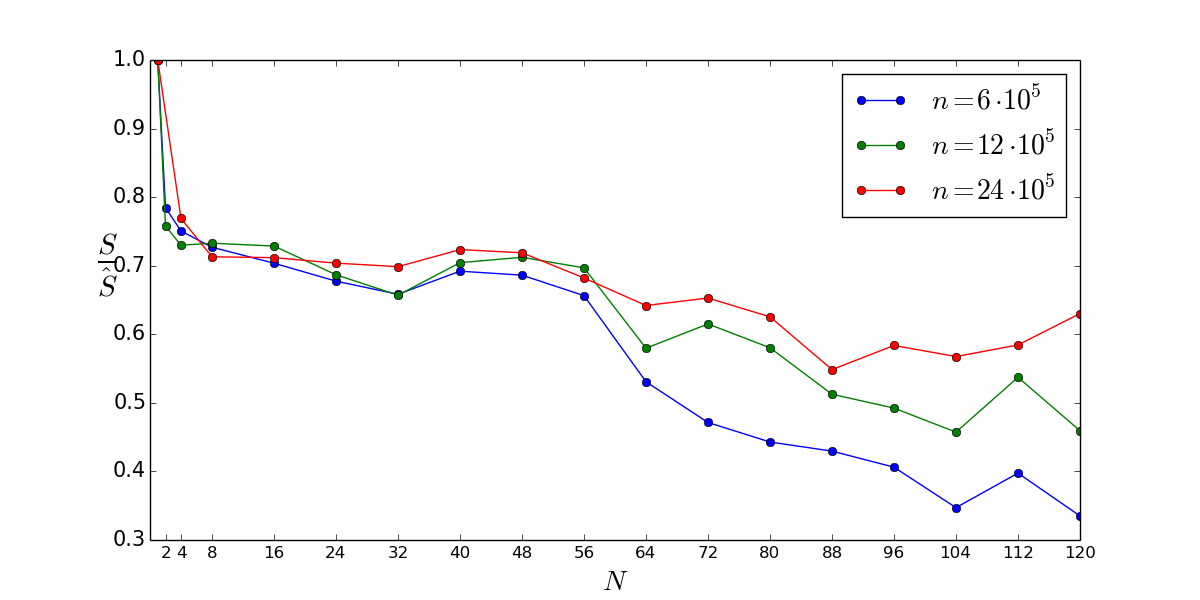
\includegraphics[scale=0.2]{SS2.png}
\end{subfigure}
\end{figure}
\end{columns}
\end{frame}
\end{comment}
\begin{frame}
\frametitle{Concluding Remarks}
\textbf{Summary}
\begin{itemize}
\item{We have proposed a parallel in time framework for optimal control based on a Parareal-preconditioned BFGS solver.}
\item{Using an example problem and an implementation we have investigated the consistency and performance of our method.}
\end{itemize}
\textbf{Extensions}
\begin{itemize}
\item{PDE}
\end{itemize}
\end{frame}
%\end{comment}
\end{document}

